
\section{From embedded spatial graphs to planar diagrams}
\label{supp:projection}
Once an embedded graph is supplied, projection changes its representation rather than its incidence. The input contract requires finite node coordinates and ordered finite three-dimensional edge polylines with endpoints at the incident vertices. The projection layer combines deterministic spherical-Fibonacci view sampling \cite{kg_keinert2015fibonacci}, spatially indexed segment queries \cite{kg_leutenegger1997str,kg_shapely} and planar-diagram encoding \cite{kg_mastin2015pdcode} within the spatial-graph framework \cite{kg_kauffman1989spatial,kg_flapan2017spatial}.

The integration distinguishes graph vertices from projection crossings, checks numerical genericity, recovers strand height from the stored three-dimensional geometry and retains the chosen projection with its PD data. Duplicate incidences are merged consistently along edge paths. These checks are designed to expose unresolved inputs rather than manufacture a valid-looking diagram. They concern the supplied piecewise-linear embedding; they do not certify its preceding reconstruction from another object.

\subsection{Generic projection sampling and selection}
\label{supp:projection_sampling}
A prescribed Euler rotation selects one view, which is still subject to the crossing and admissibility checks. Otherwise, the multi-view route uses deterministic upper-hemisphere spherical-Fibonacci/golden-angle directions \cite{kg_keinert2015fibonacci}. The three views in \SuppFigpanelref{suppfig:pdcode_to_yamada}{a} illustrate the representation change. The in-plane roll is fixed and opposite viewing directions are not separately sampled in this convention. Each candidate rotates the complete graph before projection to the $xy$ plane. This describes the intended corrected sampling procedure; it is not a claim that every historical figure was generated by an identical implementation revision.

\begin{table}[!t]
\centering\small
\begin{tabular}{p{0.27\linewidth}p{0.66\linewidth}}
\hline
\textbf{Projection event} & \textbf{Treatment}\\\hline
Overlapping or collinear projected segments & Reject the view instead of assigning artificial crossings.\\[0.35em]
Near-tangent four-incidence intersection & Reject when the cyclic order is not numerically resolved within the angular tolerance.\\[0.35em]
Unresolved strand height & For nonincident strands, reject when a reliable over/under assignment is unavailable. A genuine common graph endpoint is treated as a vertex, not as a crossing.\\[0.35em]
Accepted generic projection & Retain the complete view, crossing data and PD representation.\\\hline
\end{tabular}
\caption{\textbf{Numerical acceptance checks for a spatial-graph projection.} Invalid views are excluded rather than coerced into PD data. Acceptance is relative to the supplied piecewise-linear geometry and numerical tolerances, not an interval-arithmetic proof about uncertain input coordinates.}
\label{supptab:projection_acceptance}
\end{table}

Rejected views are recorded and skipped in a multi-view call. If none passes \SuppTabref{supptab:projection_acceptance}, projection returns an error. Among accepted candidates the selector uses the fewest crossings, breaking ties by deterministic generation order. This changes computational cost rather than the underlying supplied graph. A failure is not replaced by an abstract graph polynomial and then reported as a successful spatial evaluation.

\subsection{Crossing detection and three-dimensional over/under recovery}
\label{supp:projection_crossings}
The stored polylines, rather than straight node-to-node chords, determine the projected crossings. Each edge is decomposed into two-point segments; an STR tree generates candidates for vectorized \texttt{Shapely} intersection tests \cite{kg_shapely,kg_leutenegger1997str}. Collinear overlap is a nongeneric event. At a candidate transverse point intersection, the $z$ coordinate of each three-dimensional segment is interpolated at the projected location. Distinct heights supply the over/under assignment. An unresolved height for nonincident strands invalidates the view rather than permitting the crossing to be silently dropped. Common graph endpoints are handled through graph incidence, not confused with projection crossings.

A crossing at an internal polyline sample may be encountered through multiple adjacent segment pairs. Duplicate incidences are merged before diagram construction. The retained crossings are ordered by arclength along each original projected edge, associating each cut location with its parent edge and over/under data. Correct endpoint tangents require distinct neighboring polyline samples; a near-duplicate coordinate must not supply a spurious local direction. The resulting record supports the arc splitting in \SuppFigpanelref{suppfig:pd_code_generation}{a} and the view-specific diagrams in \SuppFigpanelref{suppfig:pdcode_to_yamada}{b}.

\begin{figure}[!t]
\centering
\includegraphics[width=\linewidth]{GeneralVersion/Figures/PDCodeGeneration.pdf}
\caption{\textbf{Planar-diagram encoding retains graph vertices and crossing information.}
\textbf{(a)} Embedded edges are cut at their ordered projected crossings; each resulting arc receives a label. \textbf{(b)} Graph vertices are serialized as counter-clockwise $V[\cdots]$ records and crossings as $X[\cdots]$ records. Crossing incidences are cyclically ordered and shifted so the overstrand occupies the evaluator's required positions. Arc labels are arbitrary identifiers; incidence, cyclic order and over/under information carry the diagrammatic meaning.}
\label{suppfig:pd_code_generation}
\end{figure}

\subsection{Arc splitting, cyclic incidence and PD serialization}
\label{supp:pd_serialization}
The ordered crossing structure is converted to discrete incidence data. In \SuppFigpanelref{suppfig:pd_code_generation}{a}, splitting at two crossings produces arcs labeled $0,1,\ldots,6$. The upper vertex is incident to arcs $3,0,2$, and the lower vertex to $4,6,3$. The outer strands are subdivided at their crossings so that each label identifies an arc between consecutive vertices or crossing objects.

A vertex record has the form $V[a_1,a_2,\ldots,a_d]$, with incidences counter-clockwise around the vertex. The two degree-three vertices therefore give $V[3,0,2]$ and $V[4,6,3]$. At a crossing, the four incidences are ordered counter-clockwise and the record starts at an overpassing incidence. The first and third entries identify the overstrand, and the second and fourth identify the understrand. The two crossings in the example are $X[4,2,5,1]$ and $X[1,5,0,6]$. The starting arc within the overpassing pair fixes a representative of the convention rather than an additional topological datum.

The complete example is
\begin{equation*}
V[3,0,2];\ V[4,6,3];\ X[4,2,5,1];\ X[1,5,0,6].
\end{equation*}
Different projections can have different crossing layouts, arc labels and PD strings. Each is an input to the invariant engine; whether their normalized values must agree depends on the admissible graph and vertex-structure setting.

\begin{figure}[!t]
\centering
\includegraphics[width=\linewidth]{GeneralVersion/Figures/PDcode_to_yamada.pdf}
\caption{\textbf{Diagram construction and invariant interpretation have different scopes.}
\textbf{(a)} Three views of one stored graph; \textbf{(b)} crossing recovery; \textbf{(c)} their PD serializations; and \textbf{(d)} the retained normalized diagram outputs. The graph has a six-valent vertex and is not subcubic. Without a common fixed rigid-vertex/ribbon structure and compatible diagram moves, the displayed outputs are not asserted to be the same unrestricted spatial-graph invariant. Their disagreement is not, by itself, proof of a changed spatial embedding or a general theorem that every higher-valence graph must give different values. Projection-consistency tests with the ambient-isotopy interpretation are performed in the admissible subcubic setting.}
\label{suppfig:pdcode_to_yamada}
\end{figure}

\section{Automating exact Yamada-invariant evaluation}
\label{supp:yamada_engine}
The accepted PD representation is passed to exact Yamada-polynomial evaluation (\Figpanelref{fig:functionality_overview}{c}). The classical polynomial distinguishes spatial information beyond abstract graph incidence \cite{kg_yamada1989,kg_mellor2018spatial}. The raw diagram polynomial is a regular-isotopy quantity and can acquire a monomial factor under Reidemeister I. The normalization used here removes that factor. In the appropriate rigid-vertex setting, the local vertex data are part of the object; in the subcubic setting the normalized quantity supplies the ambient-isotopy invariant used for multi-view tests. Different values distinguish admissible graph embeddings, while equal values need not imply equivalence. These statements concern graphs, not arbitrary changes of a spine of a handlebody.

For a nonzero raw polynomial $\Upsilon(G;Y)$, write $\mu(G)=\min\deg_Y\Upsilon(G;Y)$ and define
\begin{equation}
\overline{\Upsilon}(G;Y)=(-1)^{-\mu(G)}Y^{-\mu(G)}\Upsilon(G;Y).
\label{suppeq:yamada_normalization}
\end{equation}
The zero case is defined separately: if $\Upsilon(G;Y)=0$, then $\overline{\Upsilon}(G;Y)=0$, and $\mu(G)$ is not evaluated. This avoids taking the minimum degree of the zero polynomial. The empty graph and an isolated vertex are distinct inputs and are not identified merely because a reconstruction failed.

When view identity matters we write $G_{P_i}$. For admissible subcubic graphs, the normalized values from generic views agree, so the projection label can be suppressed. For higher valence, a graph supplied without a fixed common rigid-vertex structure is evaluated with its selected diagram and vertex order retained. Normalization alone does not establish compatibility between arbitrary cyclic orders generated at a high-valence vertex.

The retained example in \SuppFigref{suppfig:pdcode_to_yamada} contains such a vertex. Its unequal normalized outputs are consequently presented as diagram-specific results, not as a proof that normalization fails for an admissible fixed rigid-vertex object. The evaluator can process supplied PD data with high-valence vertices, while the subsequent invariant claim must respect the mathematical equivalence and encoding assumptions. This separation permits exact arithmetic without overstating what an arbitrary diagram output classifies.

\subsection{Local crossing relation and the formal resolution space}
\label{supp:local_yamada_relation}
For a crossing diagram $G_\times$, its two smoothings $G_0,G_\infty$ and vertex resolution $G_v$, the raw polynomial obeys
\begin{equation}
\Upsilon(G_\times;Y)=Y\,\Upsilon(G_0;Y)+Y^{-1}\Upsilon(G_\infty;Y)+\Upsilon(G_v;Y).
\label{suppeq:yamada_local_relation}
\end{equation}
The optimization retains this relation exactly. A direct expansion over $c$ crossings has $3^c$ histories. For the two-crossing example in \SuppFigref{suppfig:yamada_resolution_states}, the nine resolutions in panels \textbf{(b--j)} exhaust the three choices at each crossing.

Different histories can already have equal polynomial outcomes: the retained examples include pairs \textbf{(c,e)}, \textbf{(d,h)} and \textbf{(g,i)}. Equality of a final scalar value alone is not used to identify arbitrary intermediate states. The evaluator instead merges states when their remaining connectivity representation and the information needed for subsequent evaluation coincide, adding their exact weights.

\begin{figure}[!t]
\centering
\includegraphics[width=\linewidth]{GeneralVersion/Figures/YamadaResolutions.pdf}
\caption{\textbf{The three-state Yamada relation organizes exact crossing resolution.}
\textbf{(a)} A two-crossing diagram; \textbf{(b--j)} its $3^2=9$ resolution combinations with local weights $Y$, $Y^{-1}$ and $1$ according to \Eqref{suppeq:yamada_local_relation}. The retained polynomial annotations illustrate repeated outcomes, including \textbf{(c,e)}, \textbf{(d,h)} and \textbf{(g,i)}. State merging in a larger calculation requires equality of the relevant remaining connectivity data, not merely a visually similar diagram or a coincident evaluated number. The underlying Yamada relation is unchanged \cite{kg_yamada1989}.}
\label{suppfig:yamada_resolution_states}
\end{figure}

\subsection{Compiling the PD representation and removing redundancies}
\label{supp:yamada_compilation}
The PD incidence and crossing conventions are compiled before resolution. The evaluator stores each edge's endpoints and the two smoothing connections. Safe simplifications reduce unnecessary local resolution work without altering the polynomial of an admissible supplied diagram.

A cancellable Reidemeister-II bigon requires the same physical strand to pass over at both crossings. For oriented strands, the corresponding two crossing signs are opposite; alternating which physical strand passes over instead produces a twist that is not removed by this move. This distinction is essential both for explaining and for implementing the test.

\noindent\textbf{Qualification of the retained drawing.} The drawing below is unchanged from the original artwork. Its second overpass is assigned to the opposite physical strand, so the depicted two-crossing tangle is \emph{not} a valid example of Reidemeister-II cancellation. The arrow marked RII must not be read as a permissible move for these drawn overpasses. The valid cancellation condition is the same-overpassing-strand condition stated above and used in the algorithmic description below.

\begin{center}
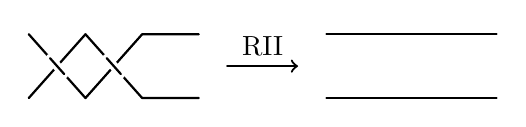
\begin{tikzpicture}[scale=0.9, line cap=round, line join=round]

% Reidemeister-II pair
\draw[line width=0.8pt]
    (0,0.45) -- (0.8,-0.45) -- (1.6,0.45) -- (2.4,0.45);
\draw[line width=0.8pt]
    (0,-0.45) -- (0.8,0.45) -- (1.6,-0.45) -- (2.4,-0.45);

% First crossing: upper strand
\draw[white,line width=3.2pt] (0.30,0.1125) -- (0.50,-0.1125);
\draw[line width=0.8pt]       (0.30,0.1125) -- (0.50,-0.1125);

% Second crossing: opposite strand is upper
\draw[white,line width=3.2pt] (1.10,0.1125) -- (1.30,-0.1125);
\draw[line width=0.8pt]       (1.10,0.1125) -- (1.30,-0.1125);

% Arrow
\draw[->,line width=0.8pt] (2.8,0) -- (3.8,0)
    node[midway,above] {$\mathrm{RII}$};

% After cancellation
\draw[line width=0.8pt] (4.2,0.45) -- (6.6,0.45);
\draw[line width=0.8pt] (4.2,-0.45) -- (6.6,-0.45);

\end{tikzpicture}

\small
Retained drawing with an incorrect second overpass: the illustrated arrow is not an allowed RII move. Valid RII removal requires the same physical strand to pass over at both crossings.
\end{center}

A valid RII cancellation preserves the raw regular-isotopy polynomial while removing two crossings. Reidemeister I changes the raw value by a monomial factor, and Reidemeister III does not reduce the crossing number. Removing an admissible pair changes the formal resolution space from $3^c$ to $3^{c-2}$.

The cancellation test searches for two crossings joined by the required pair of edges, verifies their adjacent incidence positions and compatible over/under parity, and follows the external arcs to determine the reconnection. The same physical strand must be over at both crossings. If the local pattern and reconnection are unambiguous, with the required distinct surviving endpoints, the two crossings and internal arcs are removed and the external arcs joined. Indices and smoothing connections are updated before another search. Adjacency alone is not sufficient, and the unchanged drawing is not evidence for the test's validity.

\paragraph{Organization of exact state merging}
The calculation can be described independently of a family-specific formula. First, compile and validate the diagram's incidence and crossing-resolution choices, and apply only admissible local reductions. Next, associate each surviving connectivity state with an exact Laurent-polynomial weight. Process the next crossing using the three terms of \Eqref{suppeq:yamada_local_relation}; update the corresponding connectivity and multiply the weight by $Y$, $Y^{-1}$ or $1$. Remove irrelevant label differences through the backend's canonical connectivity encoding, and combine only states with the same encoding by adding their exact weights. Once crossings are exhausted, evaluate the remaining crossing-free graph states with the graph-polynomial backend and sum their weighted contributions. Normalize the final polynomial only after the raw calculation, using the separate zero convention.

This specifies the mathematical organization of the optimization described here. The concrete compact-state encoding, canonicalization, traversal order and terminal graph evaluator are implementation choices available in the pinned source, rather than a new family-specific closed form. Time and memory depend on the number and size of distinct surviving states and polynomial coefficients, not on crossing count alone. A resource limit leaves an unavailable evaluation; it is not a valid zero and does not authorize abstract-polynomial substitution for an embedding-sensitive calculation.

\subsection{From exact evaluation to graph-family discovery}
\label{supp:yamada_discovery_bridge}
Published Yamada families illustrate the forward approach in which local structure is analyzed to obtain a recurrence or closed form. A generic evaluator permits a complementary data-driven approach: define a graph family, compute exact values, propose a relation and compare the relation with directly evaluated examples. In the subcubic families studied here, the intended workflow is
\begin{equation}
\boxed{\begin{aligned}
\text{define a spatial-graph family}&\longrightarrow\text{generate exact }\overline{\Upsilon}(G;Y)\text{ data}\\
&\longrightarrow\text{infer candidate relations}\longrightarrow\text{test additional family members}.
\end{aligned}}
\label{suppeq:yamada_discovery_bridge}
\end{equation}
A family formula is not required before obtaining the data. Conversely, a fit to those data does not establish the formula for every family member. The examples in \Figref{fig:three_theta_yamada_families} proceed from repeated motifs to commuting mixed words and ordered pure-braid words. The retrospective checks and the additional hypotheses required for all-family claims are developed in \SuppNoteref{supp:transfer_derivation}.
\FloatBarrier
